%\documentclass[12pt]{beamer}
\documentclass[handout, 12pt]{beamer}

\usetheme{default}

\usepackage{tikz}
\usepackage{graphicx}
\usepackage{hyperref}

\newcommand{\bigo}[1]{\mathcal{O}\mathopen{}\left(#1\right)\mathclose{}}
\newcommand{\br}[1]{\mathopen{}\left(#1\right)\mathclose{}}

\title{Complexity}
\subtitle{P, NP and all that}
\author{George Papamakarios}
\date{}

\begin{document}

\frame{\titlepage}

%%%%%%%%%%%%%%%%%%%%%%%%%%%%%%%%%%%%%%%%%%%%%%%%%%%%%%%%%%%%%%%%%%%%%%%%%%%%%%%%%%%%
\begin{frame}

\frametitle{What this talk is about}

\centering
\begin{minipage}{0.3\textwidth}
\begin{itemize}
\item P
\item NP
\item NP-hard
\item NP-complete
\end{itemize}
\end{minipage}

\end{frame}

%%%%%%%%%%%%%%%%%%%%%%%%%%%%%%%%%%%%%%%%%%%%%%%%%%%%%%%%%%%%%%%%%%%%%%%%%%%%%%%%%%%%
\begin{frame}

\frametitle{Decision problems}
\centering

input $\rightarrow$ \{yes, no\}

\end{frame}

%%%%%%%%%%%%%%%%%%%%%%%%%%%%%%%%%%%%%%%%%%%%%%%%%%%%%%%%%%%%%%%%%%%%%%%%%%%%%%%%%%%%
\begin{frame}<beamer:0>

\footnotesize
A decision problem is a computational problem in which we are given some \textbf{input} and we are expected to answer with a \textbf{yes} or a \textbf{no}. Some examples:
\begin{itemize}
\item[--] Given a number, is it prime?
\item[--] Given a list of numbers, do they sum to $0$?
\item[--] Given a directed graph, does it contain a cycle?
\item[--] Given a boolean formula, is it satisfiable?
\item[--] Given a program, is it syntactically correct?
\item[--] Given a program and a specification, does the program meet the specification?
\item[--] Given a proof, is it valid?
\item[--] Given a theorem, is it provable?
\end{itemize}
Of course, there are computational problems that are not decision problems, such as ``given a list of numbers, what is their sum?'', but this talk is about decision problems only.

\end{frame}

%%%%%%%%%%%%%%%%%%%%%%%%%%%%%%%%%%%%%%%%%%%%%%%%%%%%%%%%%%%%%%%%%%%%%%%%%%%%%%%%%%%%
\begin{frame}

\frametitle{Categorizing decision problems}
\centering
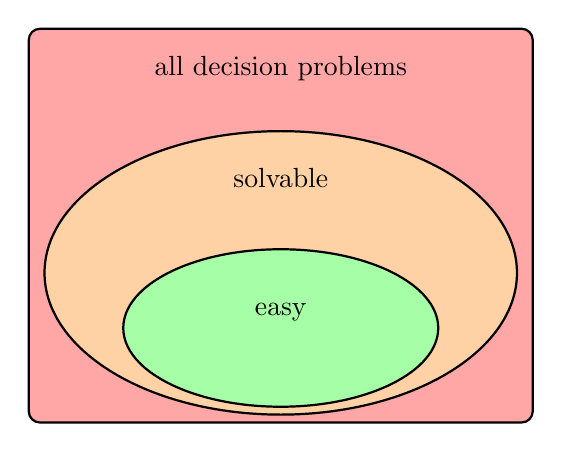
\begin{tikzpicture}

\draw<2->[rounded corners=4pt,thick,fill=red!35!white] (-3.2,0) rectangle (3.2,5);
\node<2-> at (0,4.5) {all decision problems};

\draw<3->[thick,fill=orange!35!white] (0,1.9) ellipse (3 and 1.8);
\node<3-> at (0,3.1) {solvable};

\draw<4->[thick,fill=green!35!white] (0,1.2) ellipse (2 and 1);
\node<4-> at (0,1.4) {easy};

\end{tikzpicture}

\end{frame}

%%%%%%%%%%%%%%%%%%%%%%%%%%%%%%%%%%%%%%%%%%%%%%%%%%%%%%%%%%%%%%%%%%%%%%%%%%%%%%%%%%%%
\begin{frame}<beamer:0>

\footnotesize
A remarkable result in theoretical computer science is that \textbf{not all decision problems can be solved by an algorithm}! Computability theory studies the boundary between algorithmically solvable and unsolvable problems, and it's an exciting field in its own right.
\\[0.6em]
However, even if the solution to a problem can in principle be computed by an algorithm, this doesn't necessarily mean that the problem is \textbf{solvable in practice}. If computing the solution takes more time than the lifetime of the universe, then for all practical purposes the problem is unsolvable.
\\[0.6em]
The time a problem needs in order to be solved by an algorithm, as a function of the size of the input, is called its \textbf{time complexity} (or just complexity if it's obvious we're talking about time). The complexity of a problem tells us how hard the problem is, and whether it is practically solvable or not. For example, $n$ being the size of the input, a complexity of $\bigo{n^2}$ tells us that the problem is easy (polynomial complexity), whereas a complexity of $\bigo{2^n}$ tells us that the problem is hard (exponential complexity).

\end{frame}

%%%%%%%%%%%%%%%%%%%%%%%%%%%%%%%%%%%%%%%%%%%%%%%%%%%%%%%%%%%%%%%%%%%%%%%%%%%%%%%%%%%%
\begin{frame}

\frametitle{The class P}

\begin{block}{P}
The set of decision problems that can be solved by an algorithm in \textbf{polynomial time}.
\end{block}

\end{frame}

%%%%%%%%%%%%%%%%%%%%%%%%%%%%%%%%%%%%%%%%%%%%%%%%%%%%%%%%%%%%%%%%%%%%%%%%%%%%%%%%%%%%
\begin{frame}<beamer:0>

\footnotesize
A decision problem is in P if and only if \textbf{there exists an algorithm that computes the solution in polynomial time}. For example, consider the problem:
\\[0.6em]
\textit{``Given a list of numbers, do they sum to $0$?''}
\\[0.6em]
This problem is in P. To show this, here is an algorithm that solves it:
\\[0.6em]
\textit{``Sum all numbers together, and check whether the sum is equal to zero.''}
\\[0.6em]
If the list contains $n$ numbers (size of the input), then the algorithm takes time $\bigo{n}$, which is polynomial. Hence, the problem is in P.
\\[0.6em]
To show that a problem is \textbf{not in P} is usually much harder. In order to do this, we need to show that of all algorithms that solve the problem none is polynomial, or equivalently, of all polynomial algorithms that can possibly exist, none solves the problem. We'll come back to this later.

\end{frame}

%%%%%%%%%%%%%%%%%%%%%%%%%%%%%%%%%%%%%%%%%%%%%%%%%%%%%%%%%%%%%%%%%%%%%%%%%%%%%%%%%%%%
\begin{frame}

\frametitle{Non-determinism}

\begin{block}{Non-deterministic algorithm}
An algorithm with the extra property that if it has to choose between two actions, it is allowed to execute them \textbf{both at the same time}.
\end{block}

\end{frame}

%%%%%%%%%%%%%%%%%%%%%%%%%%%%%%%%%%%%%%%%%%%%%%%%%%%%%%%%%%%%%%%%%%%%%%%%%%%%%%%%%%%%
\begin{frame}<beamer:0>

\footnotesize
A non-deterministic algorithm is an algorithm with extra power; if it has to choose between two actions, it is allowed to execute them \textbf{both at the same time}. You can think of this as follows: each time there is a choice between two things, the algorithm clones itself and one clone does the first thing while the other clone does the second thing. Then both clones run alongside in parallel. For example, here is a non-deterministic algorithm:
\\[0.6em]
\textit{``For every number in a list of $n$ numbers, either keep it or delete it. If any numbers remain at the end, add them together and report whether their sum is $0$.''}
\\[0.6em]
The algorithm makes a binary choice for every number. At the end, there are $2^n$ clones running in parallel.
\\[0.6em]
A non-deterministic algorithm returns yes if \textbf{at least one of the clones returns yes}. Otherwise it returns no. For example, the above non-deterministic algorithm will return yes if and only if there exists a non-empty subset of numbers in the list that sums to $0$. 
\\[0.6em]
Obviously, non-deterministic algorithms are not actual algorithms in the practical sense, but rather theoretical constructs. However, they are of paramount importance in the study of complexity.

\end{frame}

%%%%%%%%%%%%%%%%%%%%%%%%%%%%%%%%%%%%%%%%%%%%%%%%%%%%%%%%%%%%%%%%%%%%%%%%%%%%%%%%%%%%%%%%%%%%%%%%%%%%%%%%%%%%%%%%%%%%%%%%%%%%%%%%%%%%%%%%%%%%%%%%%%%%%%%%%%%%%%%%%%%%%%%%
\begin{frame}

\frametitle{The mouse and the cheese}

Imagine you are a mouse in front of a maze that looks like a binary tree. You want to know: \textbf{is there cheese at the other side}?
\\[0.6em]
\centering
\begin{tikzpicture}

\node at (0,0.6) {
\includegraphics[width=2.5em]{pics/mouse.jpg}};

\draw[very thick] (0,0) -- (-2,-1);
\draw[very thick] (0,0) -- (2,-1);

\draw[very thick] (-2,-1) -- (-3,-2);
\draw[very thick] (-2,-1) -- (-1,-2);
\draw[very thick] (2,-1) -- (3,-2);
\draw[very thick] (2,-1) -- (1,-2);

\draw[very thick] (-3,-2) -- (-3.5,-3);
\draw[very thick] (-3,-2) -- (-2.5,-3);
\draw[very thick] (-1,-2) -- (-1.5,-3);
\draw[very thick] (-1,-2) -- (-0.5,-3);
\draw[very thick] (3,-2) -- (3.5,-3);
\draw[very thick] (3,-2) -- (2.5,-3);
\draw[very thick] (1,-2) -- (1.5,-3);
\draw[very thick] (1,-2) -- (0.5,-3);

\node at (1.6,-3.4) {
\includegraphics[width=2.5em]{pics/cheese.jpg}};

\end{tikzpicture}


\end{frame}

%%%%%%%%%%%%%%%%%%%%%%%%%%%%%%%%%%%%%%%%%%%%%%%%%%%%%%%%%%%%%%%%%%%%%%%%%%%%%%%%%%%%
\begin{frame}<beamer:0>

\footnotesize
The mouse wants to determine whether there is cheese at the other side of the maze. To do this, a \textbf{deterministic} mouse has to visit each and every leaf of the tree. If it finds cheese at one of them, then it stops and shouts ``cheese!''. If it visits all leafs without finding cheese anywhere, then it knows there is no cheese. For a tree of depth $n$, there are $2^n$ leafs, each of which takes at most $n$ steps for the mouse to reach. Thus, the poor mouse, bound by the limits of its own determinism, has to make $\bigo{n2^n}$ steps.
\\[0.6em]
However, if the mouse is \textbf{non-deterministic}, every time it reaches a fork it can clone itself and one mouse clone can go to the left and the other mouse clone can go to the right. At some point a mouse clone will reach a leaf. If it finds cheese, full of enthusiasm it will shout ``cheese!''. If not, disappointed and tired, it will remain there in silence. If the mice hear someone shouting ``cheese!'', they will all know there is cheese at the other side of the maze. Otherwise, if after $n$ steps there is silence, all mice will know that there is no cheese.
\\[0.6em]
Allowing the mouse to be non-deterministic, the problem was solved in $\bigo{n}$! Compare this to the deterministic mouse; allowing for non-determinism can reduce exponential complexity to polynomial! This is the power of non-deterministic algorithms: \textbf{they can explore an exponential number of possibilities all at once}.

\end{frame}

%%%%%%%%%%%%%%%%%%%%%%%%%%%%%%%%%%%%%%%%%%%%%%%%%%%%%%%%%%%%%%%%%%%%%%%%%%%%%%%%%%%%%%%%%%%%%%%%%%%%%%%%%%%%%%%%%%%%%%%%%%%%%%%%%%%%%%%%%%%%%%%%%%%%%%%%%%%%%%%%%%%%%%%%
\begin{frame}

\frametitle{The class NP}

\begin{block}{NP}
The set of decision problems that can be solved by a \textbf{non-deterministic} algorithm in \textbf{polynomial time}.
\end{block}

\end{frame}

%%%%%%%%%%%%%%%%%%%%%%%%%%%%%%%%%%%%%%%%%%%%%%%%%%%%%%%%%%%%%%%%%%%%%%%%%%%%%%%%%%%%
\begin{frame}<beamer:0>

\footnotesize
A decision problem is in NP if and only if \textbf{there exists a non-deterministic algorithm that computes the solution in polynomial time}. For example, consider the problem:
\\[0.6em]
\textit{``Given a list of numbers, does any of its non-empty subsets sum to $0$?''}
\\[0.6em]
This problem is in NP. To show this, consider this algorithm:
\\[0.6em]
\textit{``For every number in the list, either keep it or delete it. If any numbers remain at the end, add them together and report whether their sum is $0$.''}
\\[0.6em]
The algorithm runs in time $\bigo{n}$, since it visits each element once. If there exists a non-empty subset of sum $0$, then one clone will find it and the algorithm will return yes. Otherwise, no clone will return yes and therefore the algorithm will return no. We have thus shown the above problem to be in NP.
\\[0.6em]
Compare this to a deterministic algorithm that checks every subset; there are $2^n$ subsets of size at most $n$, which leads to a complexity of $\bigo{n2^n}$. Again, non-determinism reduced exponential complexity to polynomial complexity. 

\end{frame}

%%%%%%%%%%%%%%%%%%%%%%%%%%%%%%%%%%%%%%%%%%%%%%%%%%%%%%%%%%%%%%%%%%%%%%%%%%%%%%%%%%%%%%%%%%%%%%%%%%%%%%%%%%%%%%%%%%%%%%%%%%%%%%%%%%%%%%%%%%%%%%%%%%%%%%%%%%%%%%%%%%%%%%%%
\begin{frame}

\frametitle{P vs NP}

Every deterministic algorithm is trivially non-deterministic, thus every problem in P is also in NP.
\begin{equation*}
P\subseteq NP
\end{equation*}

\pause

\centering
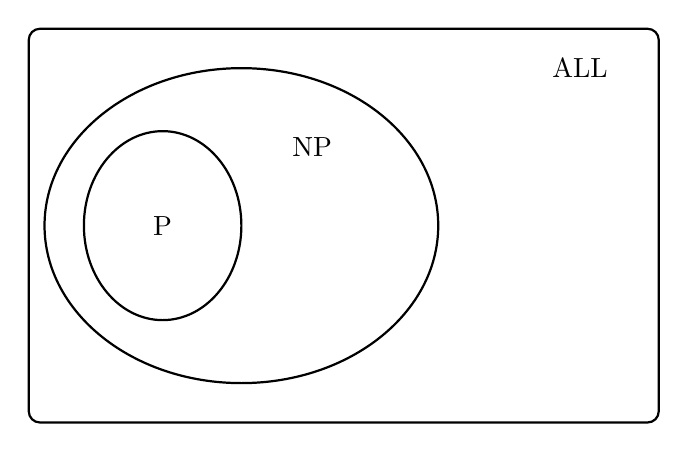
\begin{tikzpicture}

\draw<1->[rounded corners=4pt,thick] (0,-2.5) rectangle (8,2.5);
\node<1-> at (7,2) {ALL};

\draw<3->[thick] (1.7,0) ellipse (1 and 1.2);
\node<3-> at (1.7,0) {P};

\draw<4->[thick] (2.7,0) ellipse (2.5 and 2);
\node<4-> at (3.6,1) {NP};

\end{tikzpicture}

\end{frame}

%%%%%%%%%%%%%%%%%%%%%%%%%%%%%%%%%%%%%%%%%%%%%%%%%%%%%%%%%%%%%%%%%%%%%%%%%%%%%%%%%%%%%%%%%%%%%%%%%%%%%%%%%%%%%%%%%%%%%%%%%%%%%%%%%%%%%%%%%%%%%%%%%%%%%%%%%%%%%%%%%%%%%%%%
\begin{frame}

\frametitle{P vs NP}

Are there problems in NP that are not in P? That is, which of these is the case?
\begin{equation*}
P\subset NP\quad\text{ or }\quad
P = NP
\end{equation*}
\pause
\\[2em]
\centering
\color{red}{\huge We don't know!}

\end{frame}

%%%%%%%%%%%%%%%%%%%%%%%%%%%%%%%%%%%%%%%%%%%%%%%%%%%%%%%%%%%%%%%%%%%%%%%%%%%%%%%%%%%%
\begin{frame}<beamer:0>

\footnotesize
That's right, we don't know whether there are problems in NP that are not in P. Intuitively we think that allowing for non-determinism reduces complexity; but \textbf{we haven't proved it}. For all we know, it could be that non-determinism gives no extra power; it could be that the same reduction in complexity could be achieved by good old deterministic algorithms, if we are smart enough. Maybe we are not smart enough, maybe non-determinism truly gives more power; \textbf{we don't know}.
\\[0.6em]
Does it matter though? It actually \textbf{matters a lot}! There is a considerable number of real-life problems in NP that we think are not in P (but haven't proved it). If it turns out that $P\subset NP$ then pretty much nothing will change; however, if it is the case that $P = NP$ then\ldots hire bodyguards! Security and public-key cryptography rely on $P \neq NP$. It may not be an exaggeration to say that a proof for $P = NP$ could make the world dramatically different.
\\[0.6em]
The P vs NP problem is probably the most \textbf{famous open problem} in theoretical computer science; the Clay Mathematics Institute includes it in its list of $7$ Millennium Prize Problems and pays \textbf{1 million dollars} for a solution. Needless to say that numerous pseudo-solutions are published every year.

\end{frame}

%%%%%%%%%%%%%%%%%%%%%%%%%%%%%%%%%%%%%%%%%%%%%%%%%%%%%%%%%%%%%%%%%%%%%%%%%%%%%%%%%%%%%%%%%%%%%%%%%%%%%%%%%%%%%%%%%%%%%%%%%%%%%%%%%%%%%%%%%%%%%%%%%%%%%%%%%%%%%%%%%%%%%%%%
\begin{frame}

\frametitle{Reductions}

\pause
\begin{block}{Reduction}
\textbf{Transforming} some problem A to some problem B such that solving B provides a solution for A.
\end{block}

\pause
\vspace{2em}
\begin{block}{Polynomial reduction}
A reduction that can be computed in \textbf{polynomial time}.
\end{block}

\end{frame}

%%%%%%%%%%%%%%%%%%%%%%%%%%%%%%%%%%%%%%%%%%%%%%%%%%%%%%%%%%%%%%%%%%%%%%%%%%%%%%%%%%%%
\begin{frame}<beamer:0>

\footnotesize
Reducing some problem A to some other problem B means \textbf{transforming A to B such that solving B provides a solution for A}. For instance, consider these two problems:
\\[0.6em]
A = \textit{``Given a list of numbers, is any of them $0$?''}
\\[0.6em]
B = \textit{``Given a number, is it $0$?''}
\\[0.6em]
We can reduce A to B by taking all the numbers in the list and multiplying them together. Then, determining whether the product is $0$ also determines the answer to the original problem, that is whether any of the original numbers is $0$.
\\[0.6em]
Reductions are a powerful tool for \textbf{comparing problems}; if we construct a reduction from some problem A to some problem B we know we can solve, then we automatically know that we can solve A. One particular class of reductions is important for complexity: \textbf{polynomial reductions}, i.e.~reductions that can be computed in polynomial time. The reduction in the above example is polynomial, since it takes time $\bigo{n}$. If we can construct a polynomial reduction from A to B and B is in P, then we know A is in P. Conversely, if we construct a polynomial reduction from A which is not in P to B, then we know that B is not in P. Polynomial reductions are a powerful tool for \textbf{proving or disproving membership in P}, and that's why they are so important.

\end{frame}

%%%%%%%%%%%%%%%%%%%%%%%%%%%%%%%%%%%%%%%%%%%%%%%%%%%%%%%%%%%%%%%%%%%%%%%%%%%%%%%%%%%%%%%%%%%%%%%%%%%%%%%%%%%%%%%%%%%%%%%%%%%%%%%%%%%%%%%%%%%%%%%%%%%%%%%%%%%%%%%%%%%%%%%%
\begin{frame}

\frametitle{NP-hard and NP-complete}

\pause
\begin{block}{NP-hard}
The set of problems that \textbf{all} NP problems can be reduced to by a \textbf{polynomial reduction}.
\end{block}

\pause
\vspace{2em}
\begin{block}{NP-complete}
The \textbf{intersection} between NP and NP-hard.
\end{block}

\end{frame}

%%%%%%%%%%%%%%%%%%%%%%%%%%%%%%%%%%%%%%%%%%%%%%%%%%%%%%%%%%%%%%%%%%%%%%%%%%%%%%%%%%%%
\begin{frame}<beamer:0>

\footnotesize
Wouldn't it be nice if we could polynomially reduce all problems in NP to a single problem? It would be awesome. Then we could study the whole NP class by studying a single problem. We call the set of problems having this property \textbf{NP-hard}. Furthermore, if a problem is both in NP and in NP-hard, then we call it \textbf{NP-complete}.
\\[0.6em]
NP-complete problems are pretty cool; they have the property that all other NP problems can be reduced to them, and they are in NP themselves! And if we could find a polynomial time algorithm that solves some NP-complete problem, then the whole NP class collapses to P; this would immediately show that $P=NP$! In this sense, NP-complete problems are the hardest problems in NP.
\\[0.6em]
But do NP-hard problems even exist? And if NP-hard exists, does it really intersect with NP? The answer to both questions is \textbf{yes}. In fact, a staggering number of problems in NP have proved to be in NP-complete! 

\end{frame}

%%%%%%%%%%%%%%%%%%%%%%%%%%%%%%%%%%%%%%%%%%%%%%%%%%%%%%%%%%%%%%%%%%%%%%%%%%%%%%%%%%%%%%%%%%%%%%%%%%%%%%%%%%%%%%%%%%%%%%%%%%%%%%%%%%%%%%%%%%%%%%%%%%%%%%%%%%%%%%%%%%%%%%%%
\begin{frame}

\frametitle{SAT}

\begin{block}{}
Given a boolean formula, is it \textbf{satisfiable}?
\end{block}

\pause
\begin{block}{}
For example
$$\br{x\,\,\mathrm{or}\,\,y}\,\,\mathrm{and}\,\,\neg y$$
can be satisfied, by setting $x = \mathrm{true}$ and $y = \mathrm{false}$.
\end{block}

\pause
\begin{block}{}
\centering
\renewcommand{\tabcolsep}{1.5em}
\renewcommand{\arraystretch}{1}
\begin{tabular}{cc}
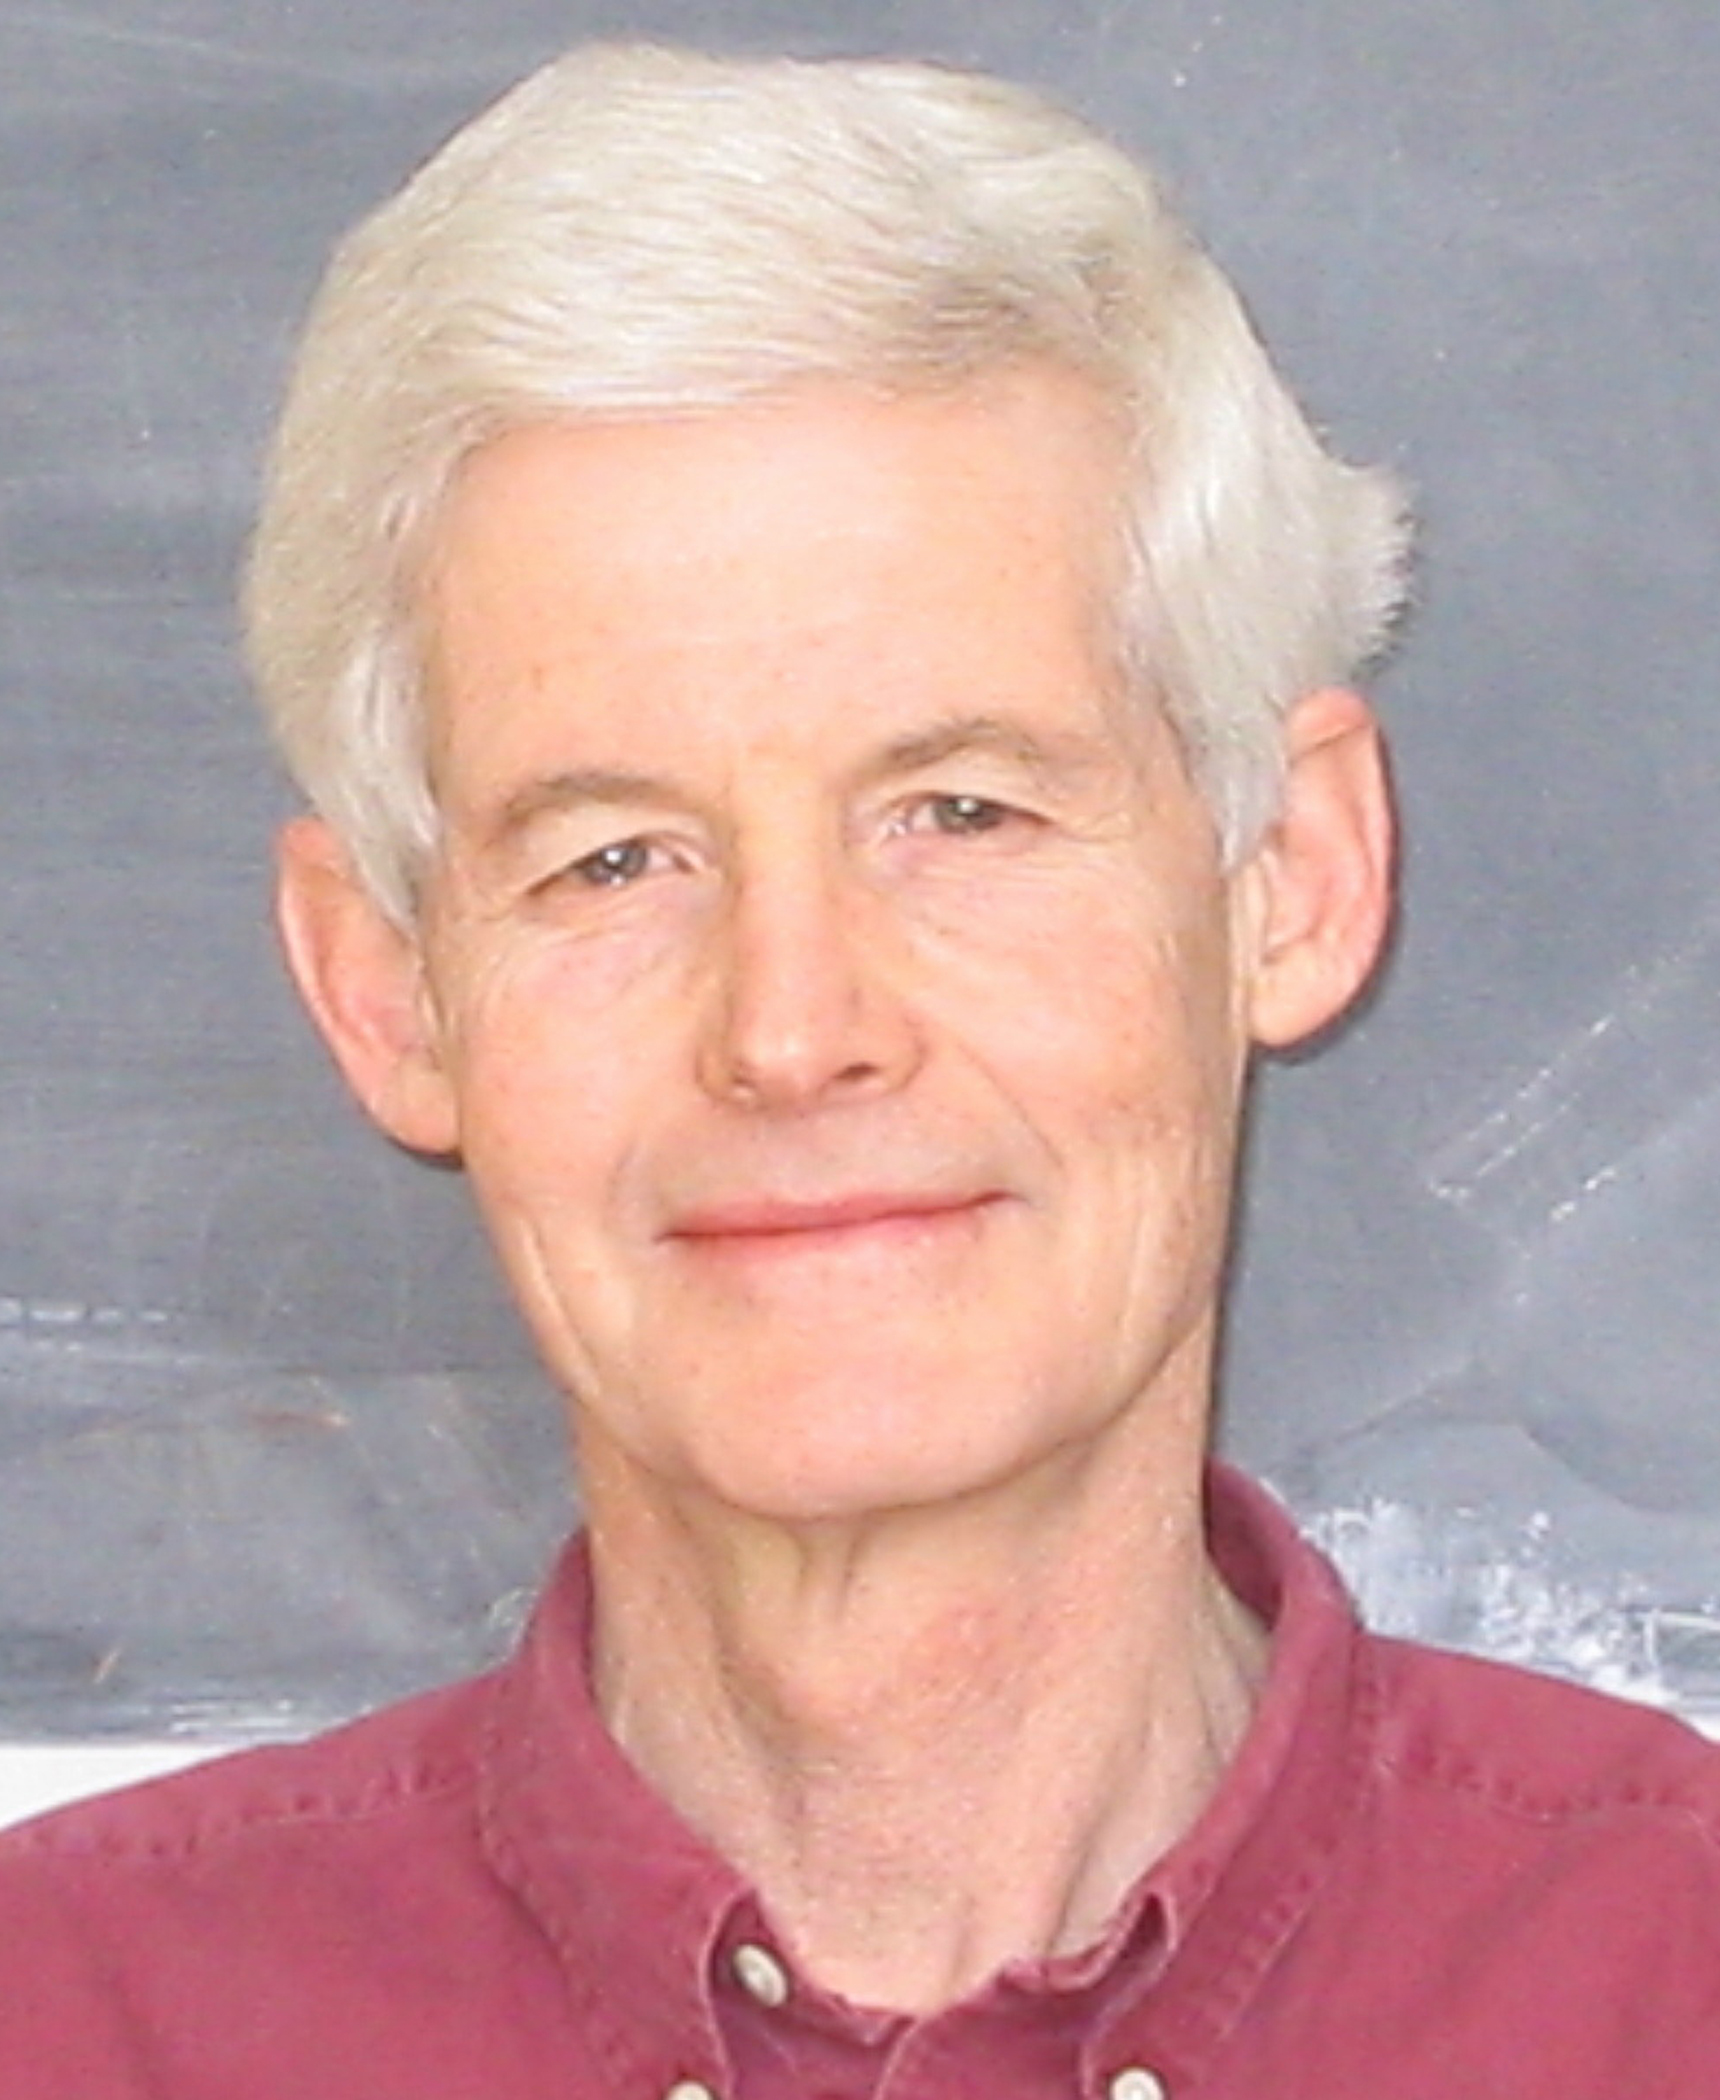
\includegraphics[width=5em]{pics/cook.jpg} & 
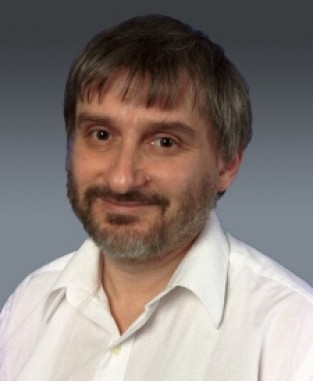
\includegraphics[width=5em]{pics/levin.jpg} \\
Stephen Cook & Leonid Levin
\end{tabular}
\end{block}

\end{frame}

%%%%%%%%%%%%%%%%%%%%%%%%%%%%%%%%%%%%%%%%%%%%%%%%%%%%%%%%%%%%%%%%%%%%%%%%%%%%%%%%%%%%
\begin{frame}<beamer:0>

\footnotesize
SAT was the first problem proved to be in NP-hard. This was proved independently by Stephen Cook in 1971 and by Leonid Levin in 1973; it is now known as the \textbf{Cook-Levin Theorem}. The proof is constructive; it literally constructs an explicit reduction from any(!) NP problem to SAT, and then shows that the reduction is indeed polynomial. Hence, SAT is proved to be in NP-hard.
\\[0.6em]
Showing that SAT is also in NP is easy. Consider the following non-deterministic algorithm:
\\[0.6em]
\textit{``For each variable in the formula, either set it to true or to false. Then evaluate the formula and report whether it's true.''}
\\[0.6em]
If $n$ is the number of variables in the formula, the above algorithm checks all $2^n$ possible assignments at once, and runs in time $\bigo{n}$. If the formula is satisfiable, one of the clones will find the satisfying assignment and the algorithm will return yes. Otherwise, no assignment is satisfying and the algorithm will return no. The algorithm solves SAT in polynomial time, hence SAT is in NP. It follows that \textbf{SAT is in NP-complete}.
\\[0.6em]
A polynomial reduction from an NP-hard problem A to some problem B immediately shows B to be in NP-hard. Having proved SAT to be in NP-hard, we are in a position to prove a whole load of other problems to be in NP-hard by reducing SAT to them.

\end{frame}

%%%%%%%%%%%%%%%%%%%%%%%%%%%%%%%%%%%%%%%%%%%%%%%%%%%%%%%%%%%%%%%%%%%%%%%%%%%%%%%%%%%%%%%%%%%%%%%%%%%%%%%%%%%%%%%%%%%%%%%%%%%%%%%%%%%%%%%%%%%%%%%%%%%%%%%%%%%%%%%%%%%%%%%%
\begin{frame}

\frametitle{Summary}

\centering
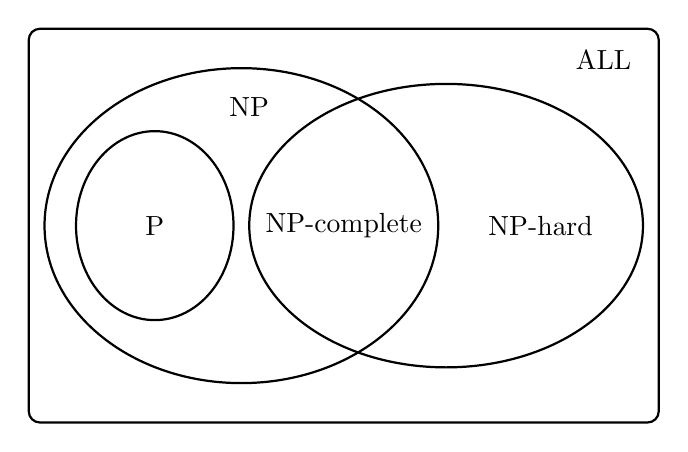
\begin{tikzpicture}

\draw<2->[rounded corners=4pt,thick] (0,-2.5) rectangle (8,2.5);
\node<2-> at (7.3,2.1) {ALL};

\draw<3->[thick] (1.6,0) ellipse (1 and 1.2);
\node<3-> at (1.6,0) {P};

\draw<4->[thick] (2.7,0) ellipse (2.5 and 2);
\node<4-> at (2.8,1.5) {NP};

\draw<5->[thick] (5.3,0) ellipse (2.5 and 1.8);
\node<5-> at (6.5,0) {NP-hard};
\node<6-> at (4,0) {NP-complete};

\end{tikzpicture}

\end{frame}

%%%%%%%%%%%%%%%%%%%%%%%%%%%%%%%%%%%%%%%%%%%%%%%%%%%%%%%%%%%%%%%%%%%%%%%%%%%%%%%%%%%%%%%%%%%%%%%%%%%%%%%%%%%%%%%%%%%%%%%%%%%%%%%%%%%%%%%%%%%%%%%%%%%%%%%%%%%%%%%%%%%%%%%%
\begin{frame}<beamer:0>

\frametitle{Sources}

\footnotesize
\textbf{Wikipedia}\\
Probably the best source out there. It has excellent articles on complexity and computability.
\\[0.6em]
\textbf{Introduction to Theoretical Computer Science}\\
An Informatics 3rd year course covering computability, complexity and lambda calculus. Materials can be found here:\\ \url{http://www.inf.ed.ac.uk/teaching/courses/itcs/}
\\[0.6em]
\textbf{Elements of the Theory of Computation}\\
A seminal book by Harry Lewis and Christos Papadimitriou. Fantastic book, it also covers finite automata and context-free grammars, in addition to complexity and computability. Currently in its 2nd edition, published by Prentice-Hall in 1997.
\\[0.6em]
\textbf{The Complexity Zoo}\\
A website with a very comprehensive list of complexity classes and their definitions. Hundreds(!) of complexity classes are listed.\\
\url{https://complexityzoo.uwaterloo.ca/Complexity_Zoo}

\end{frame}

\end{document}
